\section{FEM renderings of every load case}\label{sec:fem}
The scored solvers return safety factors and discard their fields. \src{crates/g5/src/bin/g5_fem_fields/main.rs}{\code{g5-fem-fields}}
re-solves each of the \gFemCases{} load cases of \gDesign{} on the ranking grid ($h = \gFemH$~mm) with copies of the scored models
(the whole-blade CST+DKT sandwich plate, the \code{TET10} solid tip, the \code{T6} ring with its twelve-direction sweep and the
Rayleigh--Ritz column, now with its mode) and keeps the fields: von Mises stress on a five-band sequential scale, the governing
point and the deformed shape (Figs.~\ref{fig:fem1} and~\ref{fig:fem2}). The \gFemReproduced{} scored values these solves produce
(the safety factors, the Ritz eigenvalue, the sequence ratios and the governing points) match the receipt bit for bit on the
platform of record; the tool fails if any does not.

The score models grip squeeze, guard push and teeth analytically. For those three, the figures show an independent hex8 voxel
finite-element solve on the design's own additive-manufacturing voxel field instead, reported beside the score model and not used by
it (Table~\ref{tab:hex8}).

\begin{table}[t]
\caption{Independent hex8 voxel FE against the score's analytic models (\gDesign; safety factor, required $\gReqSfYield$)}\label{tab:hex8}
\centering
\begin{tabular}{@{}lrr@{}}
\toprule
Case & Score model & Hex8 FE \\
\midrule
Grip squeeze ($\gReqGripSqN$~N) & \gFemModelGrip & \gFemHexGrip \\
Guard push ($\gReqGuardPushN$~N) & \gFemModelGuard & \gFemHexGuard \\
Serration teeth ($\gReqSnagN/\gReqPryN$~N) & \gFemModelTeeth & \gFemHexTeeth \\
\bottomrule
\end{tabular}
\end{table}

\begin{figure*}[p]
\centering
% generated by g5-release-tex from docs/g5/v<rv>/img/fem/figures.json
\begin{minipage}[t]{0.49\textwidth}\centering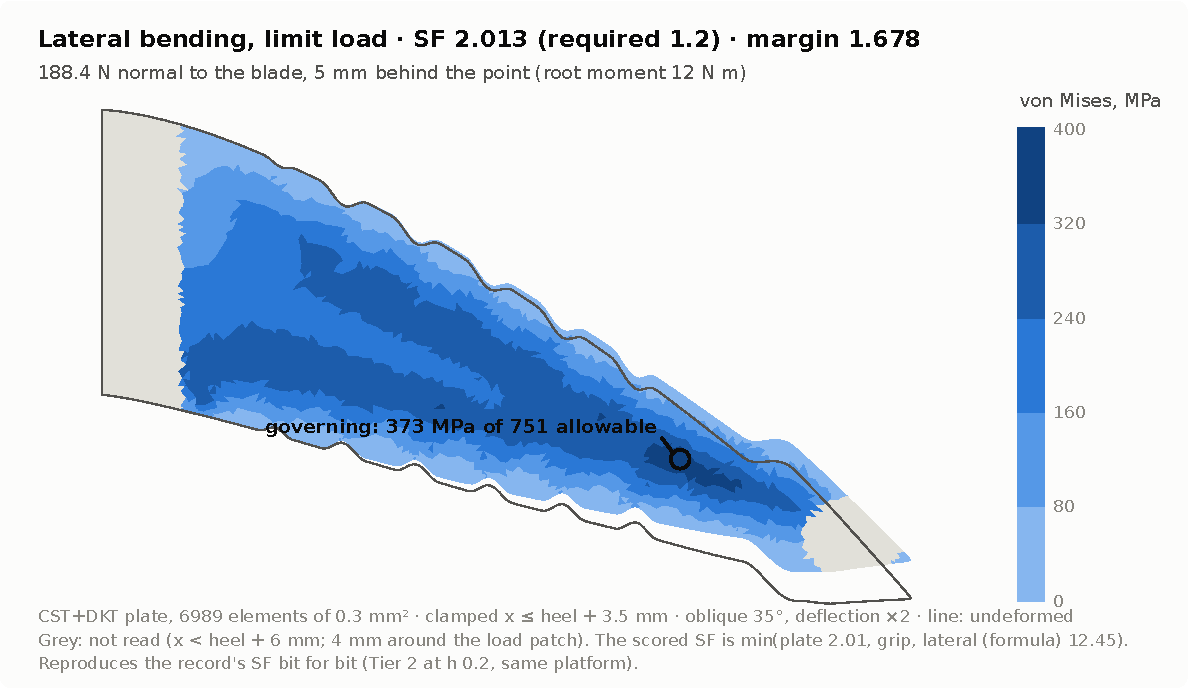
\includegraphics[width=\linewidth]{fem/lateral_limit.pdf}\\[-2pt]{\EItablefont Lateral bending, limit load: SF 2.01}\end{minipage}\hfill
\begin{minipage}[t]{0.49\textwidth}\centering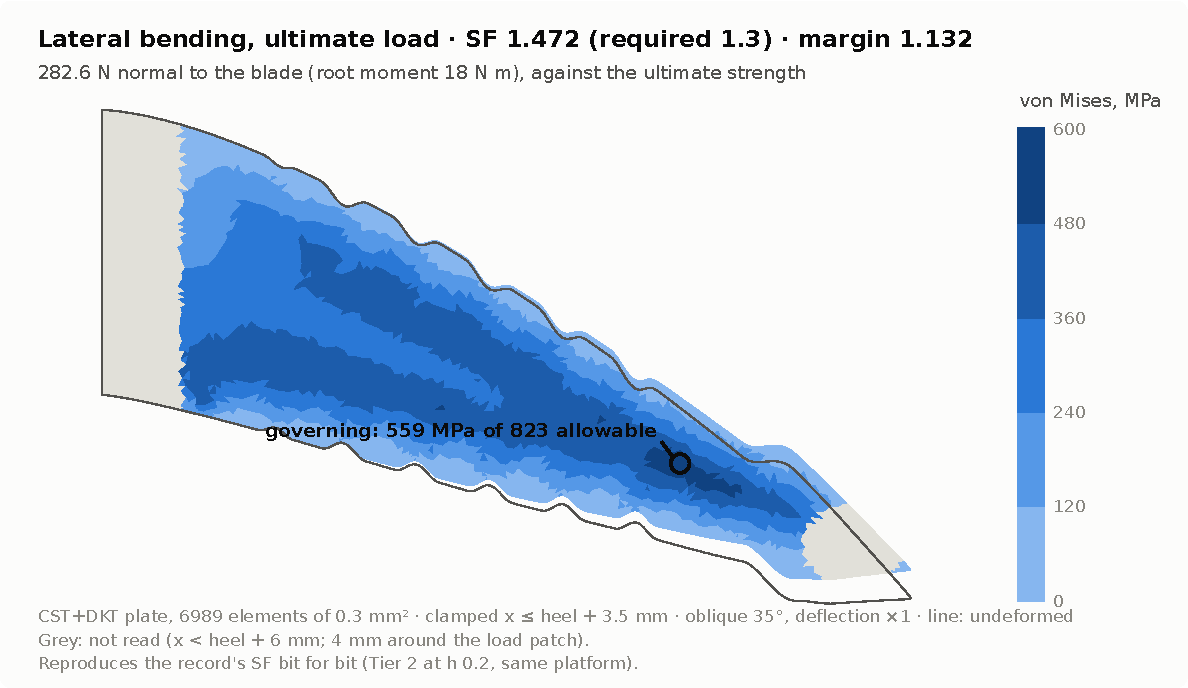
\includegraphics[width=\linewidth]{fem/lateral_ultimate.pdf}\\[-2pt]{\EItablefont Lateral bending, ultimate load: SF 1.47}\end{minipage}\\[4pt]
\begin{minipage}[t]{0.49\textwidth}\centering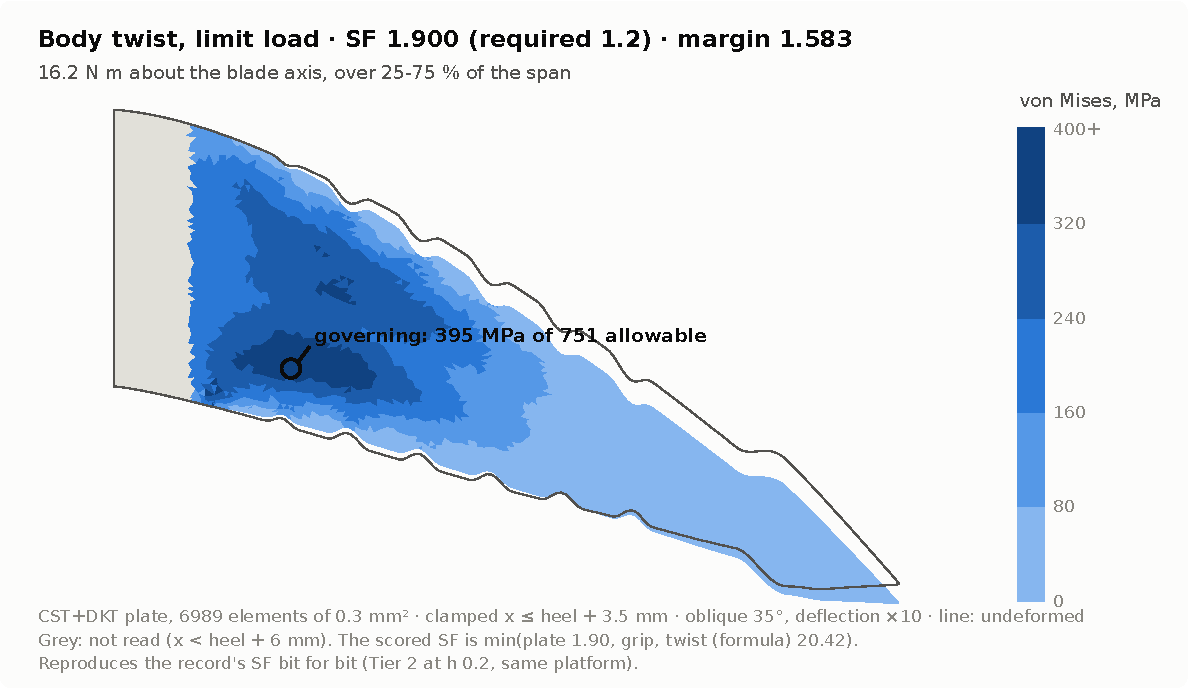
\includegraphics[width=\linewidth]{fem/twist_limit.pdf}\\[-2pt]{\EItablefont Body twist, limit load: SF 1.90}\end{minipage}\hfill
\begin{minipage}[t]{0.49\textwidth}\centering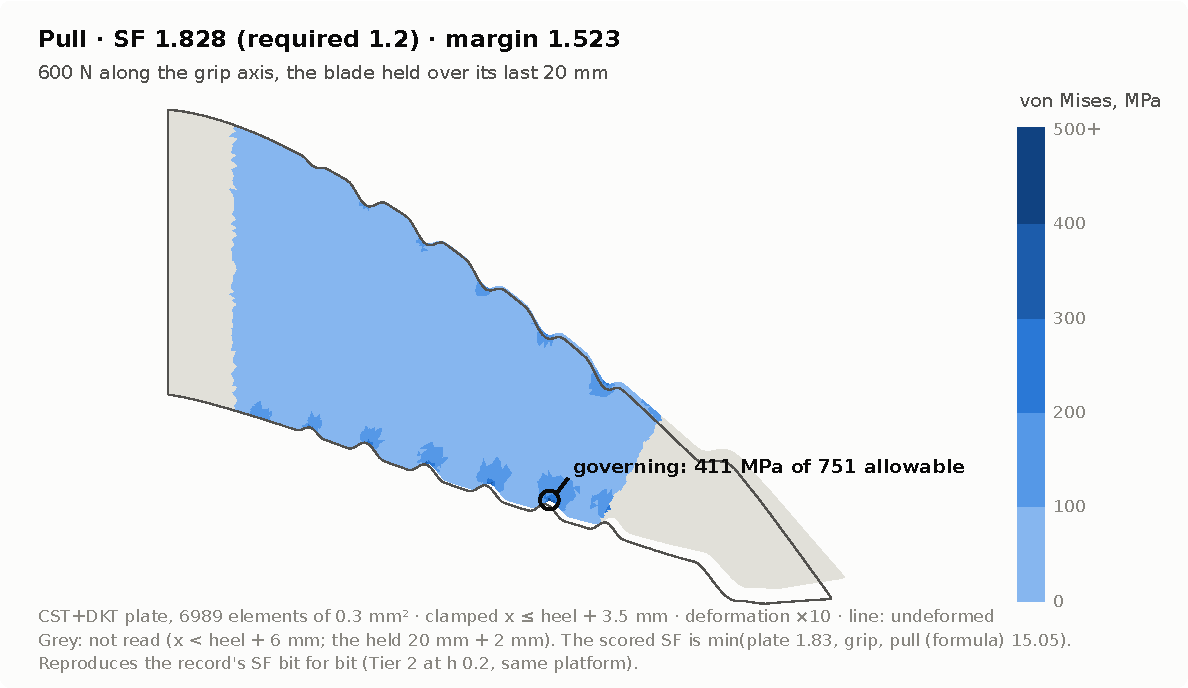
\includegraphics[width=\linewidth]{fem/pull.pdf}\\[-2pt]{\EItablefont Pull: SF 1.83}\end{minipage}\\[4pt]
\begin{minipage}[t]{0.49\textwidth}\centering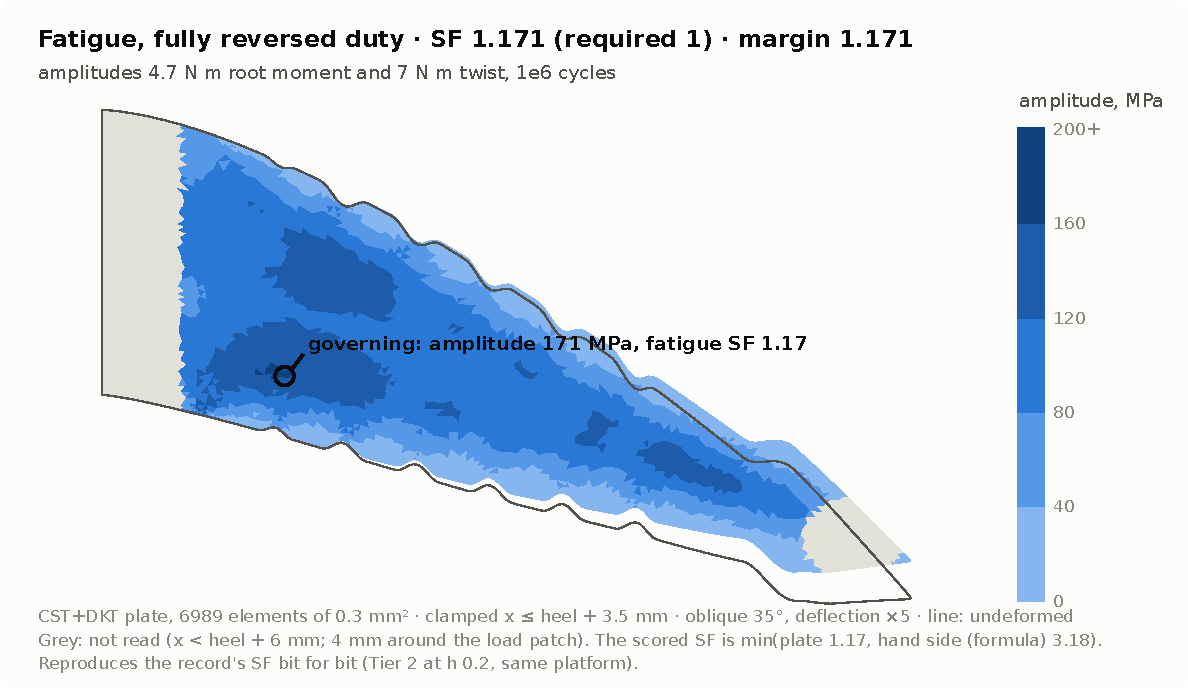
\includegraphics[width=\linewidth]{fem/fatigue.pdf}\\[-2pt]{\EItablefont Fatigue, fully reversed duty: SF 1.17}\end{minipage}\hfill
\begin{minipage}[t]{0.49\textwidth}\centering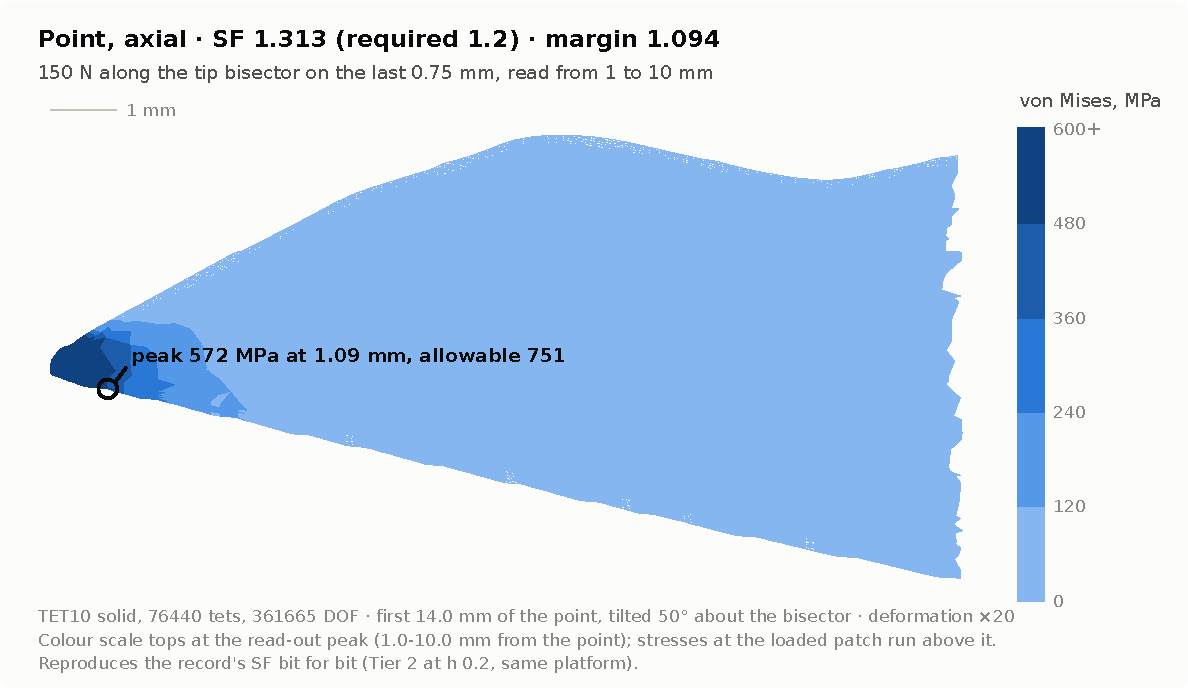
\includegraphics[width=\linewidth]{fem/tip_axial.pdf}\\[-2pt]{\EItablefont Point, axial: SF 1.31}\end{minipage}\\[4pt]
\begin{minipage}[t]{0.49\textwidth}\centering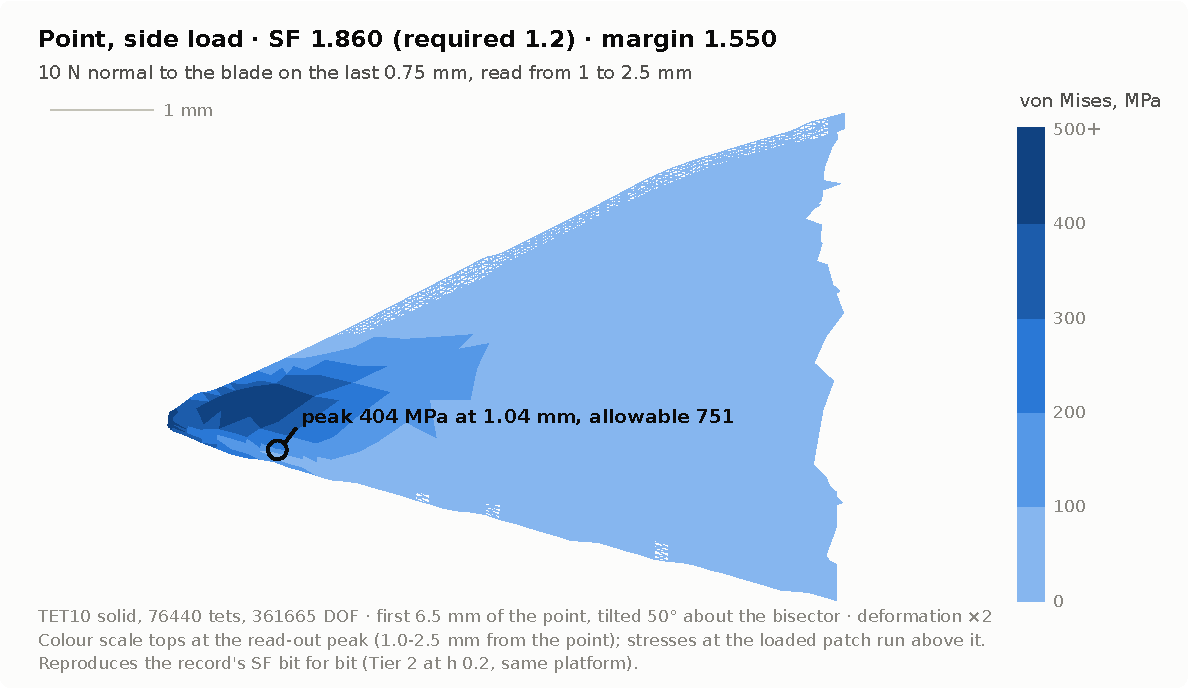
\includegraphics[width=\linewidth]{fem/tip_lateral.pdf}\\[-2pt]{\EItablefont Point, side load: SF 1.86}\end{minipage}\hfill
\begin{minipage}[t]{0.49\textwidth}\centering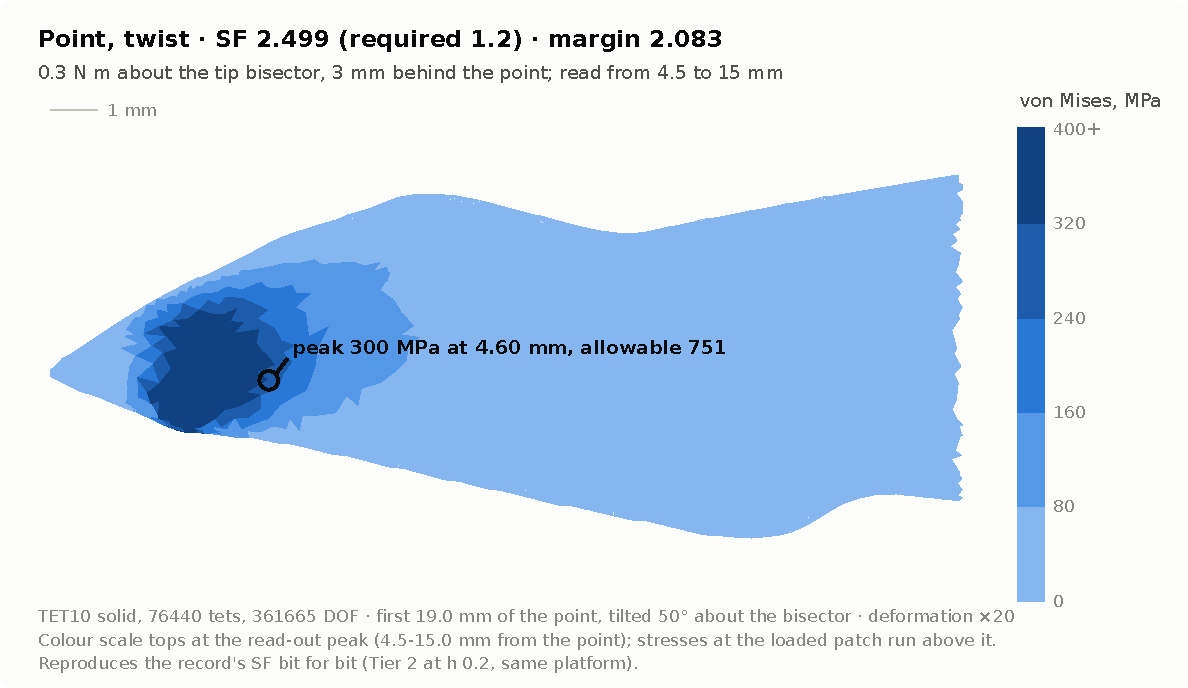
\includegraphics[width=\linewidth]{fem/tip_twist.pdf}\\[-2pt]{\EItablefont Point, twist: SF 2.50}\end{minipage}\\[4pt]

\caption{FEM renderings of the load cases of \gDesign{} (1 of 2): von Mises stress, governing point and deformed shape, as
re-solved by \code{g5-fem-fields}; each panel states its mesh, load and safety factor.}\label{fig:fem1}
\end{figure*}

\begin{figure*}[p]
\centering
% generated by g5-release-tex from docs/g5/v<rv>/img/fem/figures.json
\begin{minipage}[t]{0.49\textwidth}\centering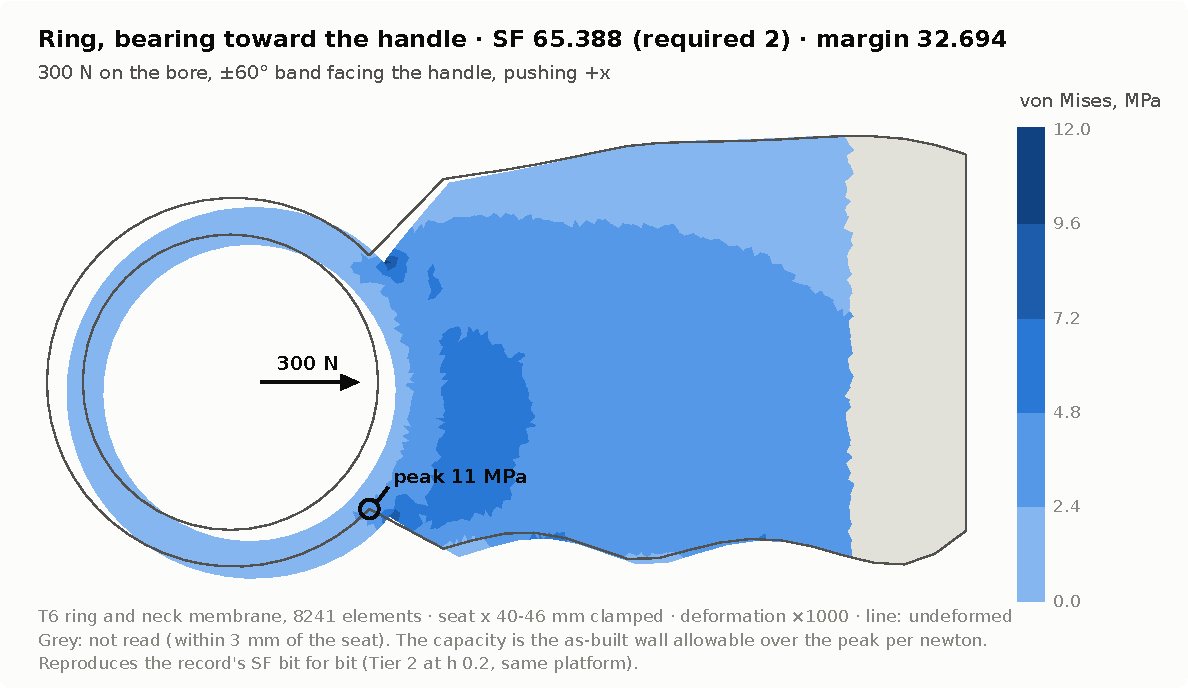
\includegraphics[width=\linewidth]{fem/ring_bearing.pdf}\\[-2pt]{\EItablefont Ring, bearing toward the handle: SF 65.39}\end{minipage}\hfill
\begin{minipage}[t]{0.49\textwidth}\centering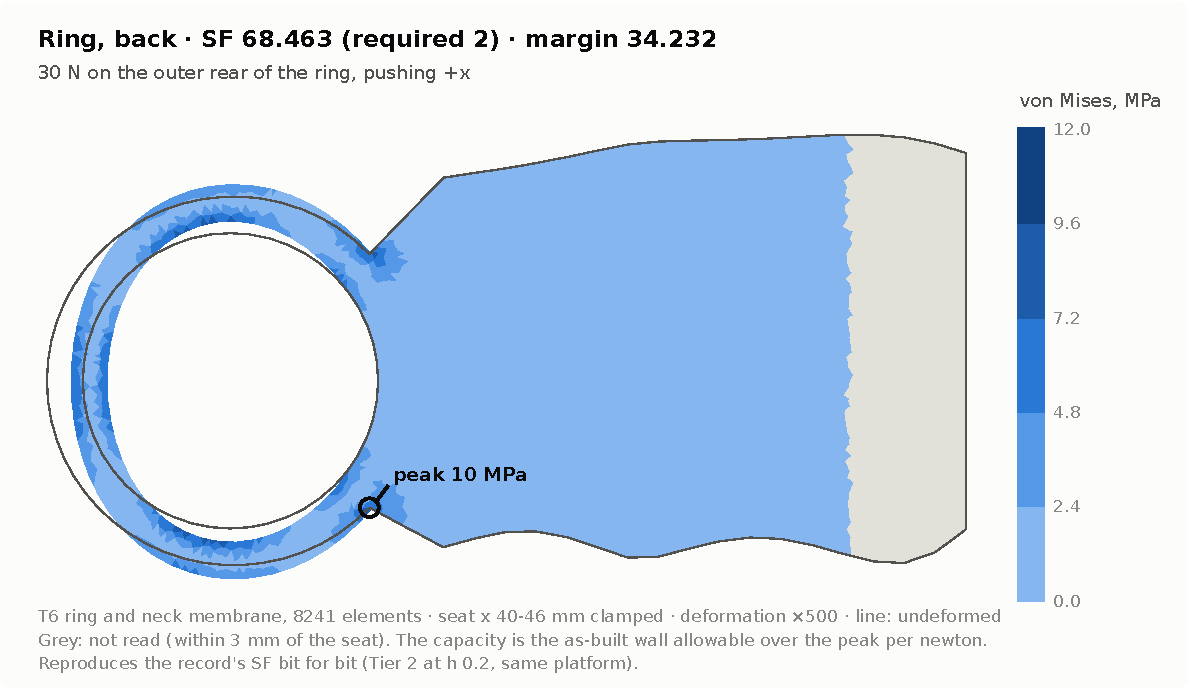
\includegraphics[width=\linewidth]{fem/ring_back.pdf}\\[-2pt]{\EItablefont Ring, back: SF 68.46}\end{minipage}\\[4pt]
\begin{minipage}[t]{0.49\textwidth}\centering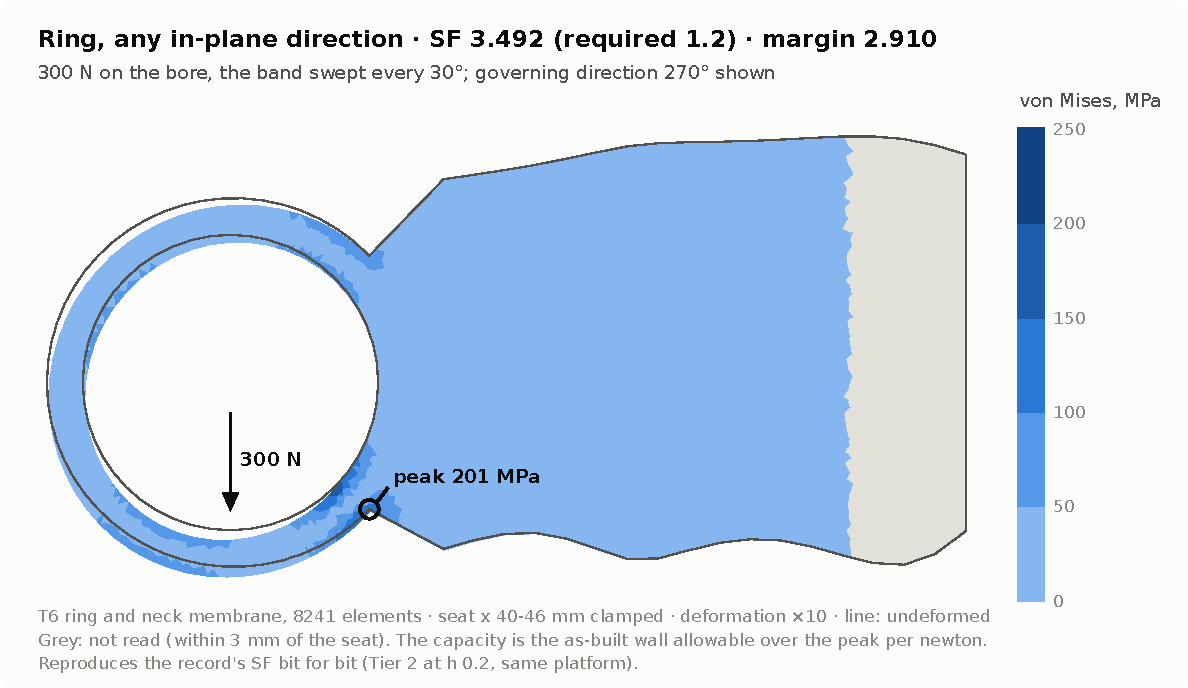
\includegraphics[width=\linewidth]{fem/ring_any_direction.pdf}\\[-2pt]{\EItablefont Ring, any in-plane direction: SF 3.49}\end{minipage}\hfill
\begin{minipage}[t]{0.49\textwidth}\centering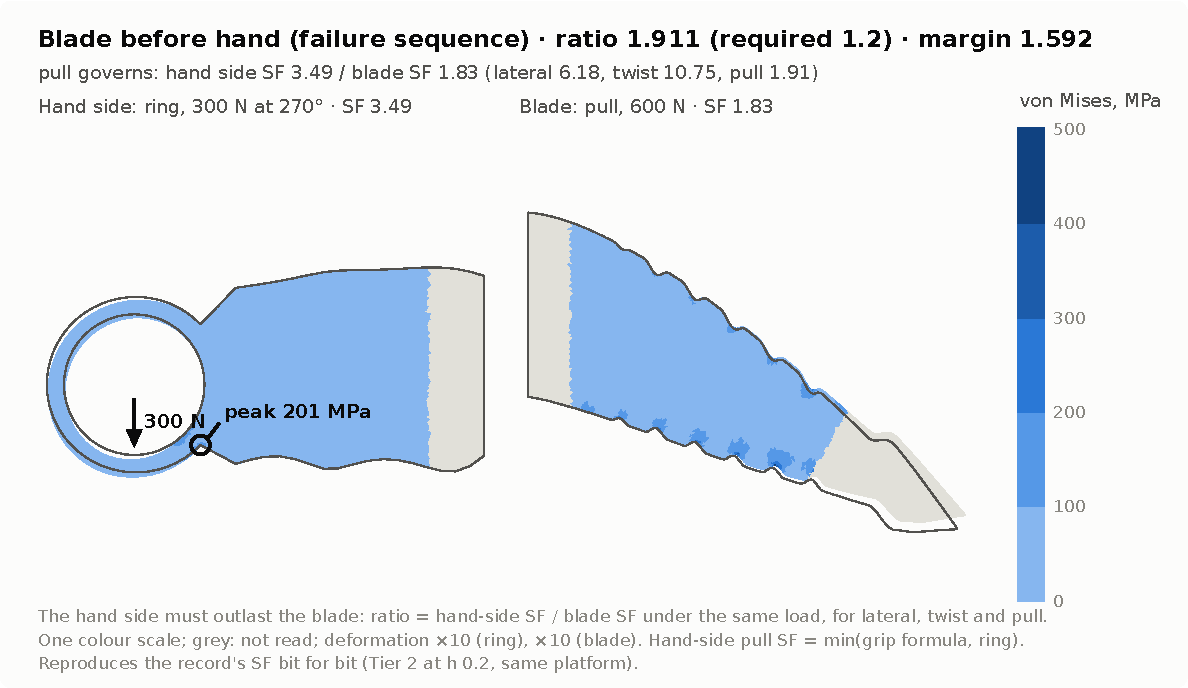
\includegraphics[width=\linewidth]{fem/sequence.pdf}\\[-2pt]{\EItablefont Blade before hand (failure sequence): SF 1.91}\end{minipage}\\[4pt]
\begin{minipage}[t]{0.49\textwidth}\centering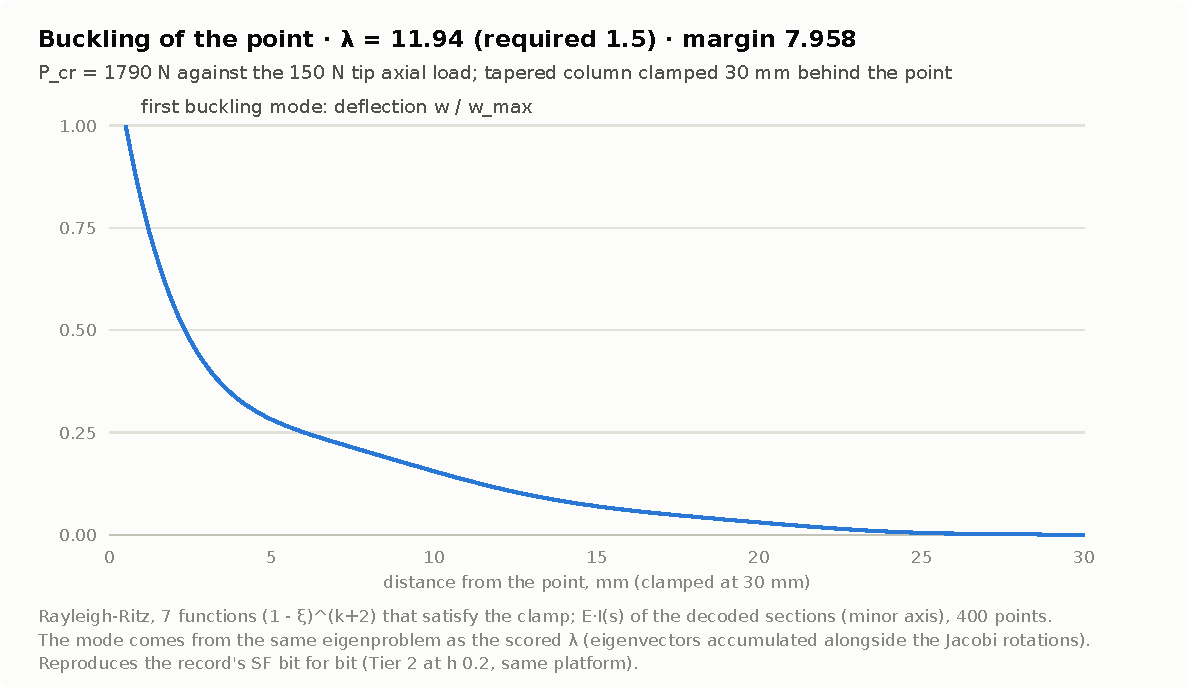
\includegraphics[width=\linewidth]{fem/buckling.pdf}\\[-2pt]{\EItablefont Buckling of the point: SF 11.94}\end{minipage}\hfill
\begin{minipage}[t]{0.49\textwidth}\centering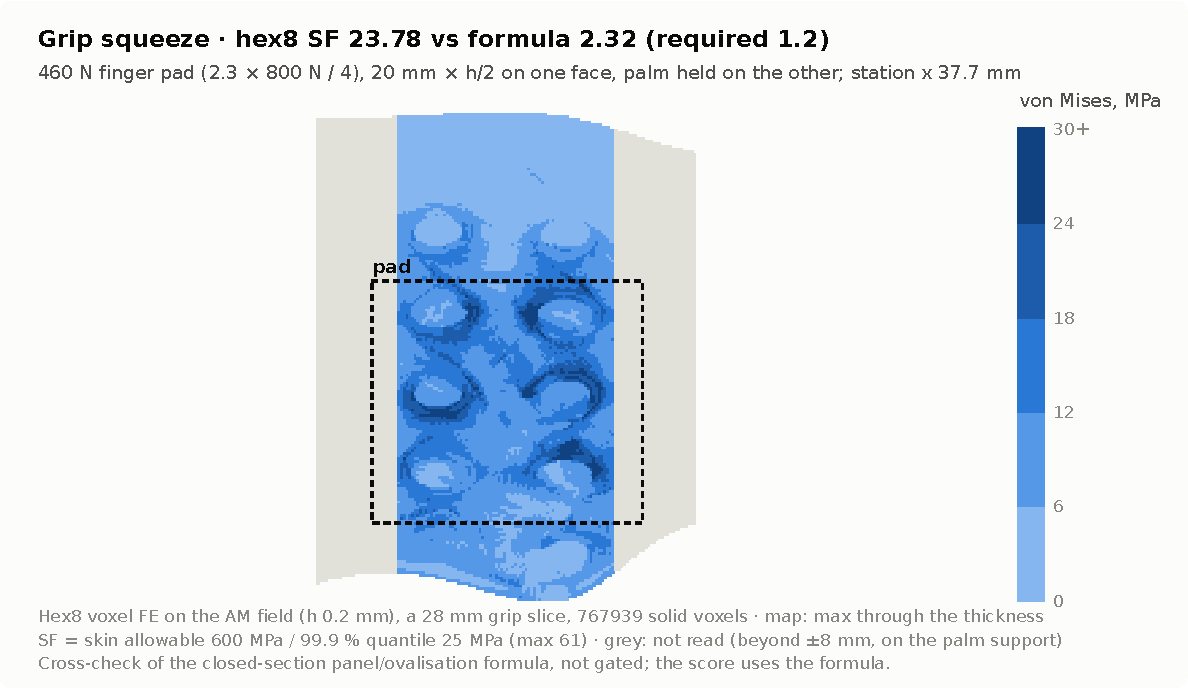
\includegraphics[width=\linewidth]{fem/grip_squeeze.pdf}\\[-2pt]{\EItablefont Grip squeeze: hex8 FE SF 23.78 (score model 2.32)}\end{minipage}\\[4pt]
\begin{minipage}[t]{0.49\textwidth}\centering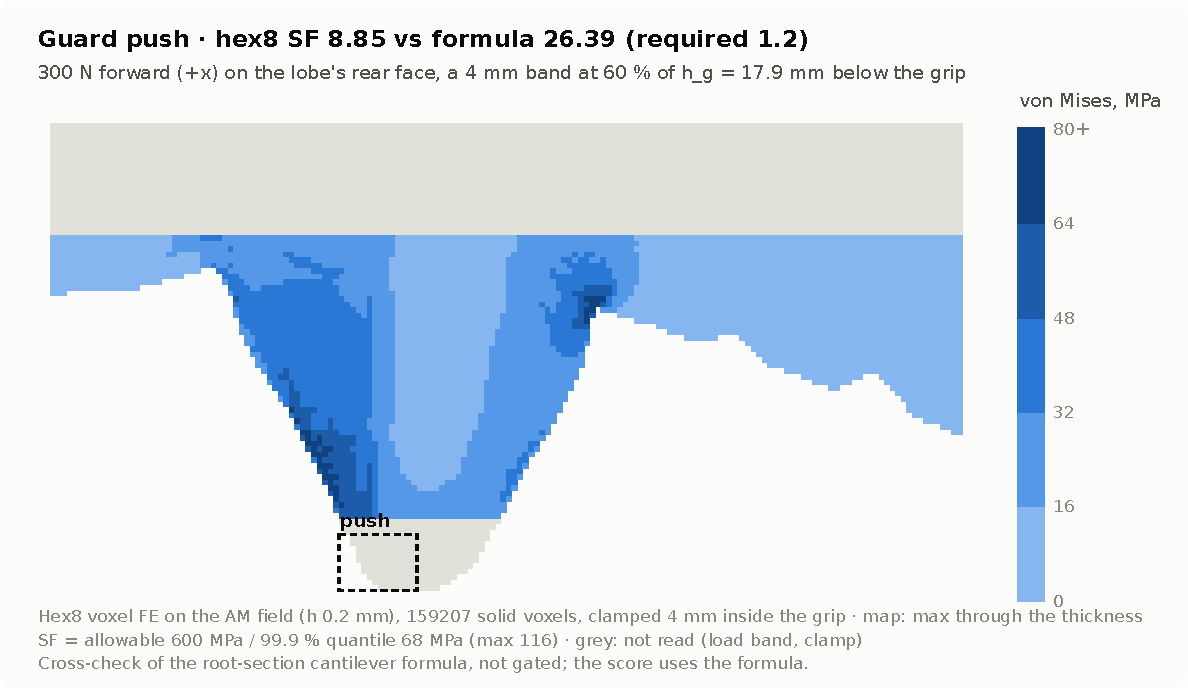
\includegraphics[width=\linewidth]{fem/guard_push.pdf}\\[-2pt]{\EItablefont Guard push: hex8 FE SF 8.85 (score model 26.39)}\end{minipage}\hfill
\begin{minipage}[t]{0.49\textwidth}\centering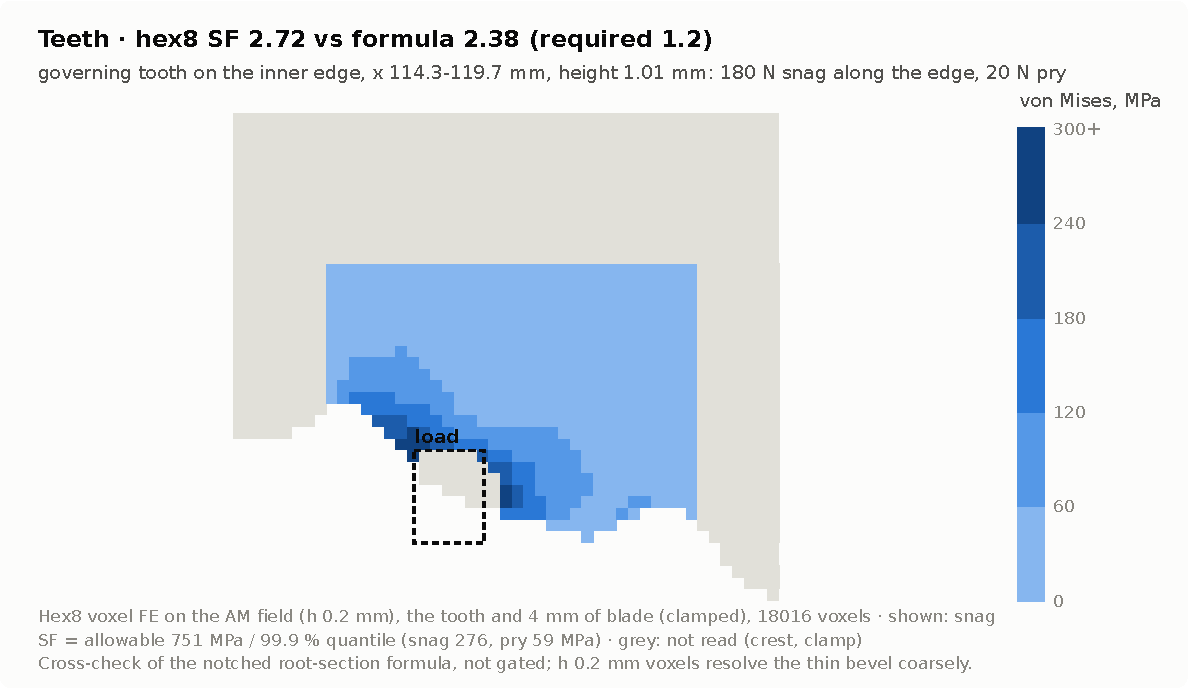
\includegraphics[width=\linewidth]{fem/teeth.pdf}\\[-2pt]{\EItablefont Teeth: hex8 FE SF 2.72 (score model 2.38)}\end{minipage}\\[4pt]

\caption{FEM renderings of the load cases of \gDesign{} (2 of 2), including the hex8 checks of the analytic cases.}\label{fig:fem2}
\end{figure*}
